\section{Fairness in machine learning}



\begin{frame}
  \begin{center} 
    {\Huge Fairness}
  \end{center}
\end{frame}


\begin{frame}
  \centering
  \begin{block}{Fairness Definitions}
    \begin{itemize}
    \item \alert{Non-discrimination}.
    \item Proportionality\footnote{\emph{Y. Liu, G. Radanovic, C. Dimitrakakis, D. C. Parkes, D. Mandal} FAT-ML 2017.}
    \item Meritocracy.
    \end{itemize}
  \end{block}
  \begin{block}{Bayesian Fairness\footnote{\emph{C. Dimitrakakis, Y. Liu, G. Radanovic, D. C. Parkes,} AAAI 2019.}}
    \Large{
      Fairness under partial information.
    }
  \end{block}

  \includegraphics[width=0.1\textwidth]{../figures/me-recent} \hspace{1em}
  \includegraphics[width=0.1\textwidth]{../figures/yang} \hspace{1em}
  \includegraphics[width=0.1\textwidth]{../figures/parkes} \hspace{1em}
  \includegraphics[width=0.1\textwidth]{../figures/goran} \hspace{1em}
  \includegraphics[width=0.1\textwidth]{../figures/deb} 
  \begin{center}
    \includegraphics[width=0.1\textwidth]{../figures/oslo}
    \hspace{1em}
    \includegraphics[width=0.1\textwidth]{../figures/ucsc}
    \hspace{1em}
    \hspace{0.1\textwidth}
    \hspace{1em}
    \includegraphics[width=0.1\textwidth]{../figures/harvard}
    \hspace{1em}
    \hspace{0.1\textwidth}
  \end{center}
  
  \note{Let us focus a bit on fairness. Fairness can mean many things, and so There are many definitions of fairness. Some relate to equity and non-discrimination, e.g. ensuring equal treatment for different genders and minorities. Some are about proportional representation. Some are about meritocracy, e.g. ensuring that the best-qualified applicants get into university. However most of these choices are not possible to satisfy simultaneously.
  
    In our with Yang Liu, David Parkes and Goran Radanovic we do not try and define a new notion of fairness. Instead, we wish to see what happens when we have only partial information. We show that by adapting a Bayesian approach, we can obtain policies that are not only inherently fairer, but that also allow us to take into account informational feedback effects when we make decisions sequentially.}
\end{frame}


\begin{frame}
  \frametitle{Bail decisions}
  \centering

  \begin{columns}
    \begin{column}{0.5\textwidth}
      \begin{tikzpicture}
        \node[label={$x,z$}] at (-1,2) (person)
        {\includegraphics[width=0.2\columnwidth]{../figures/zuckerberg}};
        \node[label=$\pi$] at (0,0) (judge) {\includegraphics[width=0.3\columnwidth]{../figures/judge}};
        \draw[->] (person) -- (judge);
        \uncover<2->{
          \node[label=$a_1$] at (-2,-2) (jail) {\includegraphics[width=0.3\columnwidth]{../figures/jail}};
          \draw[->] (judge) -- (jail);
        }
        \uncover<3->{
          \node[label=$a_2$] at (2,-2) (bail) {\includegraphics[width=0.3\columnwidth]{../figures/bail}};
          \draw[->] (judge) -- (bail);
        }
        \uncover<4->{
          \node[label=$y_1$] at (-2,-4) (trial) {\includegraphics[width=0.3\columnwidth]{../figures/trial}};
          \draw[->] (jail) -- (trial);
        }
        \uncover<5->{
          \draw[->] (bail) -- (trial);
        }
        \uncover<6->{
          \node[label=$y_2$] at (2,-4) (arrest) {\includegraphics[width=0.3\columnwidth]{../figures/handcuffs}};
          \draw[->] (bail) -- (arrest);
        }
      \end{tikzpicture}
    \end{column}
    \begin{column}{0.5\textwidth}
      \only<1-7>{
        \begin{itemize}
        \item $x$ - features
        \item $z$ - sensitive features
        \item $a$ - action
        \item $y$ - outcome
        \end{itemize}
      }
      \only<8>{\includegraphics[width=0.8\columnwidth]{../figures/judge-fairness}}
      \uncover<2->{\[\pi(a \mid x) \tag{policy}\]}
      \uncover<4->{\[P_\param(x,y,z) \tag{model}\]}
      \uncover<7->{\[U(a,y) \tag{utility}\]}

    \end{column}
  \end{columns}

  \note<1>{Let us begin with a simple example. In the US system of justice, an accused is presented before a judge. The accused has some observable features x, as well as some possibly sensitive features z such as ethnicity or gender.}
  \note<2>{ Based on what the judge sees, she uses a policy pi to make a decision. Should the defendant be kept in jail until trial?}
  \note<3>{Or should they be let go?}
  \note<4>{If they are kept in jail, then they almost invariably go to trial.}
  \note<5>{They may also go to trial if they are freed...}
  \note<6>{But they may also flee or commit another crime.}
  \note<7>{Typically, the judge makes the decision by weighing the risk against a utility function that measures the cost of keeping an innocent in prison versus the cost of them committing another crime.}
\end{frame}

\begin{frame}
  \frametitle{The USA COMPAS System\footnote{Pro-publica, 2016}}
  Assigns a \alert{risk score} $a_t$ to defendant $x_t$.
  \begin{figure}[H]
    \begin{columns}
      \begin{column}{0.5\textwidth}
        \centering
        \def\svgwidth{.95\columnwidth}
        \input{../figures/risk-scores-black.pdf_tex}
        Black
      \end{column}
      \begin{column}{0.5\textwidth}
        \centering
        \def\svgwidth{0.95\columnwidth}
        \input{../figures/risk-scores-white.pdf_tex}      
        White
      \end{column}
    \end{columns}
    \label{fig:risk-bias}
    \caption{Apparent bias in risk scores towards black versus white defendants.}
  \end{figure}
\end{frame}


\subsection{Group fairness and conditional independence}
\begin{frame}
  \only<1>{
    \includegraphics[width=\columnwidth]{../figures/imrs}
    \\\scriptsize{Washington Post, 2016}
  }
  \only<2>{
    \includegraphics[width=\columnwidth]{../figures/imrs-risk}
    \\\scriptsize{Pro-publica, 2016}
  }
  \begin{columns}
    \begin{column}{0.3\textwidth}
      \begin{itemize}
      \item[$y$] Result.
      \item[$a$] Assigned score.
      \item[$z$] Race.
      \end{itemize}
    \end{column}
    \begin{column}{0.7\textwidth}
      \begin{align}
        \Pr_\param^\pi(y \mid a, z) &= \Pr_\param^\pi(y \mid a) \tag{\alert<1>{calibration}}\\
        \Pr_\param^{\pi}(a \mid y, z) &= \Pr_\param^{\pi}(a \mid y) \tag{\alert<2>{balance}}
      \end{align}
    \end{column}
  \end{columns}
  \note<1>{
    In the US, there is a system called COMPAS, which assigns a risk score from 1-10 to defendants. If we imagine that it is only the system that acts, and the judge simply makes a decision using the system score, then the score corresponds to the system action. This score informs the judge about whether or not somebody is at risk of recidivism. A typical test to see if the system works well is calibration: what is the probability of somebody committing an offence under different scores? We can see that the system is quite well-calibrated and that the calibration is the same for both black and white americans. This notion of fairness (calibration) implies that the outcome is independent of race given the action - so that the action is entirely predictive of the outcome.}
  \note<2>{However, a recent study showed a different effect. Black people that did not reoffend had an approximately equal probability of obtaining a high or low score, while black people that reoffended had significantly higher scores that those that did not. For white people, however, this was not the case. Reoffending whites had equal probability of being assigned a high score, while those that did not reoffend had overwhelmingly lower scores. This notion of fairness (balance) implies that our decision should be independent of race if we know the outcome. In hindsight, it is obvious that decisions cannot be simultaneously fair in both senses, as they imply two different type of independence. }


\end{frame}



\begin{frame}
  \frametitle{The value of a policy}
  \begin{block}<1->{Fairness metrics: balance}
    \begin{equation}
      F_{\textrm{balance}}(\param, \pol)
      \defn
      \sum_{y, z, a}
      |\Pr_\param^\pol(a \mid y, z) - \Pr_\param^\pol(a  \mid y)|^2
    \end{equation}
  \end{block}
  \begin{block}<2->{Utility: Classification accuracy}
    \[
      U(\param, \pol) = \Pr_\param^\pol (y_t = a_t)
    \]
  \end{block}
  \begin{block}<3->{Use $\lambda$ to trade-off utility and fairness}
    \begin{equation}
      \label{eq:combined-value}
      V(\lambda, \param, \pol) = (1 - \lambda) \overbrace{U(\param, \pol)}^{\textrm{utility}} - \lambda \underbrace{F(\param, \pol)}_{\textrm{unfairness}}
    \end{equation}
  \end{block}
  \note<1>{Of course, we care not only about fairness with respect to race, but also about utility: we would like our predictions to be accurate. For that reason, if we say theta describes the environment, then the value of our policy can be seen as the convex combination between a utility term and a fairness violation term.}
  \note<2>{The fairness violation term simply expresses how far away from e.g. balance our decision rule is. This can be done like in this example, where we use the square difference between the probabilities of the same action under different conditionings on the sensitive variable.}
  \note<3>{The utility can be something simple, such as the classification utility, by taking $U$ to be the identity function. Then the $I$ term is 1 when we have a correct classification, and the term is the }
\end{frame}

\begin{frame}
  \frametitle{Model uncertainty}
  \begin{theorem}
    A decision rule in the form of a lottery, i.e.
    \[
      \pi(a \mid x) = p_a
    \]
    can be the only way to satisfy balance for all possible $\param$.
  \end{theorem}

  \begin{block}{Possible solutions}
    \begin{itemize}
    \item Marginalize over $\param$ ("expected" model)
    \item Use Bayesian reasoning
    \end{itemize}
  \end{block}
  \note{The discussion here has focused on the case where we are talking about a specific probability distribution $P_\theta(x,y,z)$ from which the data is generated. However, we never know this distribution. Because of this, if we want to be fair with respect to e.g. balance for every possible model of the world, we need to essentially run a lottery: assign a fixed probability to every possible decision. This clearly is far from optimal in terms of utility. So, what can we do? There are two options. The first is to marginalise over the parameters to get an expected model of the world and optimise according to that. The second, which is what we propose, is to use Bayesian reasoning.}
\end{frame}


\begin{frame}<1,2>[label=fairness:setting]
  \frametitle{The setting}
  \only<1,2>{
    \begin{block}{Bayesian modelling of uncertainty}
      \begin{itemize}
      \item Model family $\cset{P_\param(x, y, z)}{\param \in \Param}$
      \item Prior belief $\bel_0(\param)$.
      \item Data $D \sim P_\param(x, y,z)$.
      \item Posterior belief $\bel(\param) \defn \bel_0(\param \mid D)$.
      \end{itemize}
    \end{block}
  }
  \only<2,3,4>{
    \begin{block}{The Bayesian value of a policy}
      \begin{equation}
        \label{eq:combined-value}
        V(\lambda, \bel, \pol) \defn \sum_{\param \in \Param} V(\lambda, \param, \pol) \bel(\param).
      \end{equation}
      \only<article>{This is simply the expected value of our policy over each possible parameter $\theta$, with respect to the belief $\bel$.}
    \end{block}
  }
  \only<3>{
    \begin{block}{Optimisation with stochastic gradient ascent}
      \[
        \nabla_\pol V(\lambda, \bel, \pol)
        = \int_{\Param} \nabla_\pol V(\lambda, \param, \pol) \dd \bel(\param).
      \]
    \end{block}
  }
  \only<4>{
    \begin{block}{Sequential setting}
      \begin{align*}
        \bel_t(\param) &= \bel_0(\param \mid x_{1:t-1}, z_{1:t-1}, a_{1:t-1}, y_{1:t-1})\\
        \max_\pol & \E^\pol_{\bel_1} \sum_{t=1}^T V(\lambda, \bel_t, \pol)
      \end{align*}
    \end{block}
  }
  \only<5>{
    \begin{block}{Dynamic programming}
      \begin{align*}
        \val^*(\bel_t) &\defn \sup_{\pol_t} \overbrace{\E^{\pol_t}_{\bel_t} \left[(1 - \lambda) U_t - \lambda F_t\right]}^{\textrm{current value}}
                         + \underbrace{\sum_{\bel_{t+1}} \val^*(\bel_{t+1}) \Pr_{\bel_t}^{\pol_t} (\bel_{t+1})}_{\textrm{future value}}
      \end{align*}
    \end{block}
  }
  \only<6>{
    \begin{block}{Posterior sampling}
      \begin{align*}
        \hat{\Param}_t &\sim \bel^k_t,
        &\pol_t &= \max_p \E^\pol_{\hat{\Param}_t} [(1 - \lambda) U_t - \lambda F_t]\\
        a_t &\sim \pol(a \mid x_t), & y_t \mid x_t &\sim P_\param(y_t \mid x_t)
      \end{align*}
    \end{block}
  }
  \note<1>{In the Bayesian setting, we assume that the world can be described by one of a set of possible models, and we assign some prior probability $\beta_0$ to each one of them. After we obtain some data $D$ from the world, we calculate a new distribution representing our posterior belief $\bel(\param)$.}
  \note<2>{Now, instead of looking at the value of our policy for a specific parameter $\param$, we calculate the average value of the policy with respect to our posterior distribution. This automatically takes into account our uncertainty.}
    \note<3>{In order to implement the algorithm in practice, we perform stochastic gradient descent, by sampling models from the posterior and calculating the gradient for each model. This can be done because the gradient of the expectation is equal to the expectation of the gradient. For comparison with the marginal model, we use the same gradient descent algorithm, but replace the sampling by the marginal calculation.}
  \note<4>{Of course, in an online setting, the data is not seen at once. Instead, observe $x_t$, make a decision $a_t$, and then obtain a new $x_{t+1}$. For the problem at hand, if our decision was to grant bail, then we also get to see the outcome $y_t$, otherwise we do not. Our goal is to maximise the value of the policy over time.}
  \note<5>{This optimisation problem can be solved through dynamic programming, where the optimal value for any belief $\bel_t$ is simply the expected value of the policy for that belief, plus the expected cumulative value in the future.}

\end{frame}




\begin{frame}
  \frametitle{Synthetic data}
  \centering
    \centering
    \mbox{
    \setlength \fwidth {0.3\textwidth}
    \hspace{-2em}
    % This file was created by matlab2tikz.
%
%The latest updates can be retrieved from
%  http://www.mathworks.com/matlabcentral/fileexchange/22022-matlab2tikz-matlab2tikz
%where you can also make suggestions and rate matlab2tikz.
%a

\begin{tikzpicture}

\begin{axis}[%
width=0.951\fwidth,
height=0.75\fwidth,
at={(0\fwidth,0\fwidth)},
scale only axis,
xmode=log,
xmin=1,
xmax=100,
xminorticks=true,
xlabel style={font=\color{white!15!black}},
xlabel={},
title={$\lambda = 0$},
ymin=5,
ymax=7,
ylabel style={font=\color{white!15!black}},
ylabel={V},
axis background/.style={fill=white}
]
\addplot [color=mycolor1, line width=2.0pt, forget plot]
  table[row sep=crcr]{%
1	5.43561523059217\\
2	5.90370595362012\\
3	5.86193877425643\\
4	6.1974251447707\\
5	6.37538745144895\\
6	6.29084098710727\\
7	6.37533818756081\\
8	6.50213010808347\\
9	6.5991724386949\\
10	6.52046523295858\\
11	6.72543938736623\\
12	6.79086221447693\\
13	6.73720035131321\\
14	6.73338708212267\\
15	6.72543680895541\\
16	6.69340595276163\\
17	6.7374401920428\\
18	6.76459636329051\\
19	6.81917107124367\\
20	6.81961739074537\\
21	6.80848937741292\\
22	6.76496273549776\\
23	6.81943224558462\\
24	6.82707956663492\\
25	6.82513922838762\\
26	6.80872080097762\\
27	6.8194279261825\\
28	6.8189260277632\\
29	6.80836851035401\\
30	6.80853114441057\\
31	6.81931954445528\\
32	6.73856115284411\\
33	6.73816264740434\\
34	6.73350236577814\\
35	6.70687112292105\\
36	6.6785416628419\\
37	6.67686803452494\\
38	6.73847232580075\\
39	6.81942547936638\\
40	6.82688492791769\\
41	6.82666694620967\\
42	6.82685885290022\\
43	6.82704019063763\\
44	6.82689924230517\\
45	6.82677823960367\\
46	6.8270597587393\\
47	6.8194560097514\\
48	6.82689843014005\\
49	6.82701602901863\\
50	6.82681169930566\\
51	6.81949797532045\\
52	6.82669354234299\\
53	6.81943329511497\\
54	6.82651491512469\\
55	6.82704770792639\\
56	6.82679743590289\\
57	6.82658758155496\\
58	6.82669828218253\\
59	6.82660948782845\\
60	6.82669798274291\\
61	6.8265894448791\\
62	6.82677142197074\\
63	6.82681491374407\\
64	6.82666114793132\\
65	6.80855816288338\\
66	6.81943481045244\\
67	6.82660396672482\\
68	6.82386355702123\\
69	6.81947471789097\\
70	6.82700074175287\\
71	6.82693449357647\\
72	6.82709850214994\\
73	6.82660499877464\\
74	6.82697649873285\\
75	6.82670593695921\\
76	6.82675415174255\\
77	6.82687238452097\\
78	6.82695391513762\\
79	6.82698434483159\\
80	6.82686631929662\\
81	6.82688791087935\\
82	6.82646811164595\\
83	6.82644252014829\\
84	6.82665183718036\\
85	6.82669758685249\\
86	6.82676665652696\\
87	6.82695751973057\\
88	6.82658946086894\\
89	6.82655885737069\\
90	6.82664771118609\\
91	6.82677188302957\\
92	6.82669723134228\\
93	6.82649131899508\\
94	6.82694362296807\\
95	6.82701100800417\\
96	6.82689276186491\\
97	6.82697942973237\\
98	6.8265959260873\\
99	6.82685566499548\\
100	6.82661794251553\\
};
\addplot [color=mycolor2, dashed, line width=3.0pt, forget plot]
  table[row sep=crcr]{%
1	5.41383459952623\\
2	6.03977740818528\\
3	6.34445896962323\\
4	6.36360081485984\\
5	6.5327140246455\\
6	6.54312011538435\\
7	6.60180812138142\\
8	6.73373741924754\\
9	6.73566894837812\\
10	6.79427286043087\\
11	6.79651547742057\\
12	6.81745557776205\\
13	6.82361089403465\\
14	6.82453008513155\\
15	6.81832088322606\\
16	6.78744690174988\\
17	6.8245307167606\\
18	6.82360223044389\\
19	6.82320123869577\\
20	6.82664800772996\\
21	6.82680811620926\\
22	6.82647925470442\\
23	6.82692086547104\\
24	6.8269265759928\\
25	6.82693425257449\\
26	6.8268229060682\\
27	6.82700552417735\\
28	6.82667175358748\\
29	6.82668179704755\\
30	6.82696045898621\\
31	6.82660833511297\\
32	6.82680589726841\\
33	6.82671589421294\\
34	6.82682294359754\\
35	6.82701707308604\\
36	6.82650493640409\\
37	6.82699220517708\\
38	6.82668021066387\\
39	6.82672209879424\\
40	6.82681624339904\\
41	6.82673440179816\\
42	6.82689211021934\\
43	6.82677720152432\\
44	6.82694542985608\\
45	6.82666056532852\\
46	6.82671478552557\\
47	6.82693547661731\\
48	6.82672478318047\\
49	6.82677490664466\\
50	6.82656216462366\\
51	6.82648634438907\\
52	6.82704568401014\\
53	6.826862274337\\
54	6.82707378292588\\
55	6.82701064453263\\
56	6.82655872230876\\
57	6.82680284995162\\
58	6.82675484205814\\
59	6.82669898677491\\
60	6.8269587402534\\
61	6.82659491807925\\
62	6.8270850859566\\
63	6.82673295666194\\
64	6.82699550615579\\
65	6.82685223576769\\
66	6.82671348441515\\
67	6.82673202844262\\
68	6.82712820153405\\
69	6.82689184429809\\
70	6.82683272593571\\
71	6.82648201507614\\
72	6.82674866309257\\
73	6.82671747591638\\
74	6.82699024215261\\
75	6.82717941910823\\
76	6.82694493886605\\
77	6.8267239335274\\
78	6.82696730470131\\
79	6.82694340122485\\
80	6.82682976358288\\
81	6.82660119141053\\
82	6.82686412764447\\
83	6.82699084765003\\
84	6.8267722735916\\
85	6.82674429780571\\
86	6.82694302876559\\
87	6.82675714405635\\
88	6.82696031751509\\
89	6.82689255300199\\
90	6.82702023326717\\
91	6.82696488326549\\
92	6.82660850972417\\
93	6.8268004525055\\
94	6.82679611886495\\
95	6.82682594191007\\
96	6.82686735298234\\
97	6.82672601577022\\
98	6.82680403091386\\
99	6.82704486981606\\
100	6.8267221923614\\
};
\end{axis}
\end{tikzpicture}%
    \hspace{-2em}
    % This file was created by matlab2tikz.
%
%The latest updates can be retrieved from
%  http://www.mathworks.com/matlabcentral/fileexchange/22022-matlab2tikz-matlab2tikz
%where you can also make suggestions and rate matlab2tikz.
%
%
\begin{tikzpicture}

\begin{axis}[%
width=0.951\fwidth,
height=0.75\fwidth,
at={(0\fwidth,0\fwidth)},
scale only axis,
xmode=log,
xmin=1,
xmax=100,
xminorticks=true,
xlabel style={font=\color{white!15!black}},
xlabel={},
title={$\lambda = 0.5$},
ymin=-0.5,
ymax=2,
axis background/.style={fill=white}
]
\addplot [color=mycolor1, line width=2.0pt, forget plot]
  table[row sep=crcr]{%
1	1.49482275002729\\
2	1.55189801874307\\
3	1.83882282524574\\
4	1.52676135329926\\
5	1.52250894001475\\
6	1.50531193637208\\
7	1.49370990313388\\
8	1.37096218428233\\
9	1.69252155043745\\
10	1.55460080897603\\
11	1.77758287824582\\
12	1.78571302890306\\
13	1.54890376428204\\
14	1.71169980084041\\
15	1.76677542583961\\
16	1.79953306466444\\
17	1.82405896323217\\
18	1.80562258987096\\
19	1.80346372081525\\
20	1.80490522019214\\
21	1.80251864349951\\
22	1.7995840760207\\
23	1.79674085586432\\
24	1.806276571382\\
25	1.81194647146786\\
26	1.82251291652957\\
27	1.80498094116489\\
28	1.8272796312303\\
29	1.80961959279471\\
30	1.81460137914183\\
31	1.81914916541425\\
32	1.81392379924514\\
33	1.8175432722861\\
34	1.8201478669015\\
35	1.81322273333226\\
36	1.81866634019849\\
37	1.81584318931693\\
38	1.82674652739832\\
39	1.80998697957214\\
40	1.81282450380663\\
41	1.82359620006886\\
42	1.82111823610408\\
43	1.82290286766311\\
44	1.81848658484606\\
45	1.82597066631328\\
46	1.81211306569529\\
47	1.82229032524054\\
48	1.81015879277648\\
49	1.82773686379265\\
50	1.81919753307513\\
51	1.81588515919281\\
52	1.81601964781797\\
53	1.81749265215332\\
54	1.82007077847615\\
55	1.82443336078475\\
56	1.82566220552982\\
57	1.82280628482688\\
58	1.83010292007432\\
59	1.82074163362279\\
60	1.81866781943321\\
61	1.82007236165932\\
62	1.82851746138336\\
63	1.81651773830087\\
64	1.81292309805879\\
65	1.81097040505865\\
66	1.82112946548917\\
67	1.81770401450192\\
68	1.82937997687998\\
69	1.81678649459996\\
70	1.8165514209844\\
71	1.82296124397186\\
72	1.81862636466603\\
73	1.82650919211409\\
74	1.81607019489911\\
75	1.81867067516648\\
76	1.81455612740102\\
77	1.81867226688053\\
78	1.81606266049731\\
79	1.81975419210626\\
80	1.8199782675556\\
81	1.82408715716298\\
82	1.81743782363045\\
83	1.81223449479776\\
84	1.82717780566641\\
85	1.81912057558481\\
86	1.8172207355233\\
87	1.82568116472211\\
88	1.81790553467899\\
89	1.81656810711344\\
90	1.82428308742398\\
91	1.8302964899591\\
92	1.8235600515568\\
93	1.82461711494186\\
94	1.81752760149805\\
95	1.82427771424488\\
96	1.81013748370312\\
97	1.81434628986094\\
98	1.81752237732997\\
99	1.82299730857796\\
100	1.82163132633734\\
};
\addplot [color=mycolor2, dashed, line width=3.0pt, forget plot]
  table[row sep=crcr]{%
1	0.200825888532816\\
2	-0.18008397338503\\
3	-0.223529206493137\\
4	-0.0753925034742253\\
5	0.929582939469821\\
6	0.676750152052953\\
7	1.02527985927929\\
8	1.1907138620247\\
9	1.2237426133549\\
10	1.06210547603728\\
11	1.39678777894161\\
12	1.40974585704355\\
13	1.46876264509228\\
14	1.28575761797557\\
15	1.14882024066358\\
16	1.46377660532148\\
17	1.56963239593687\\
18	1.66907185300346\\
19	1.72286071590441\\
20	1.71545125972188\\
21	1.72076857522247\\
22	1.70977648241448\\
23	1.71421934606972\\
24	1.81961918396706\\
25	1.82486972192735\\
26	1.82205160751454\\
27	1.82970447855445\\
28	1.81975762676593\\
29	1.82608890642267\\
30	1.82790882921885\\
31	1.82305138404279\\
32	1.8251774473024\\
33	1.82180970765009\\
34	1.82535183629553\\
35	1.81491795840182\\
36	1.81139862864023\\
37	1.81469578968229\\
38	1.82336600035984\\
39	1.81964088422403\\
40	1.81156044832757\\
41	1.810193776878\\
42	1.81604224661703\\
43	1.81250494134455\\
44	1.81608869175998\\
45	1.8282763978939\\
46	1.81991287660889\\
47	1.81582197002685\\
48	1.8216328147671\\
49	1.81509662525265\\
50	1.81967603345366\\
51	1.82217581494403\\
52	1.81614879299987\\
53	1.82145119528924\\
54	1.82274949930973\\
55	1.81087216488805\\
56	1.82123830998816\\
57	1.82383525525647\\
58	1.82396221554174\\
59	1.81879833466988\\
60	1.82491278694981\\
61	1.81620584157348\\
62	1.81404426119364\\
63	1.81664144185502\\
64	1.82267074046262\\
65	1.81879699133598\\
66	1.82336546099748\\
67	1.82165386661804\\
68	1.82023091505951\\
69	1.81012488462726\\
70	1.81501540952032\\
71	1.81181672885677\\
72	1.81254029915353\\
73	1.81600596980627\\
74	1.82931752912828\\
75	1.82015694163513\\
76	1.82358452377752\\
77	1.82866674935601\\
78	1.81692298347132\\
79	1.81944525961421\\
80	1.81664892791178\\
81	1.81442168852228\\
82	1.81792302272156\\
83	1.81625638592239\\
84	1.81487418368066\\
85	1.81950552074845\\
86	1.82379573251609\\
87	1.82325367665394\\
88	1.81973949148139\\
89	1.82191418084967\\
90	1.82040245967622\\
91	1.81445589110821\\
92	1.8240198622246\\
93	1.82666876362131\\
94	1.82016060196285\\
95	1.81832870479655\\
96	1.81289773601116\\
97	1.81923026308184\\
98	1.81644826216325\\
99	1.8285673621865\\
100	1.82098487160116\\
};
\end{axis}
\end{tikzpicture}%
%%% Local Variables:
%%% mode: latex
%%% TeX-master: t
%%% End:

    \hspace{-2em}
    % This file was created by matlab2tikz.
%
%The latest updates can be retrieved from
%  http://www.mathworks.com/matlabcentral/fileexchange/22022-matlab2tikz-matlab2tikz
%where you can also make suggestions and rate matlab2tikz.
%
%
\begin{tikzpicture}

\begin{axis}[%
width=0.951\fwidth,
height=0.75\fwidth,
at={(0\fwidth,0\fwidth)},
scale only axis,
xmode=log,
xmin=1,
xmax=100,
xminorticks=true,
xlabel style={font=\color{white!15!black}},
xlabel={},
title={$\lambda = 1$},
ymin=-3,
ymax=-0,
axis background/.style={fill=white}
]
\addplot [color=mycolor1, line width=2.0pt, forget plot]
  table[row sep=crcr]{%
1	-0.0079538799589155\\
2	-0.029543354739046\\
3	-0.0433687510715851\\
4	-0.0267997530098269\\
5	-0.0552496970950875\\
6	-0.0426903095165145\\
7	-0.0679414709532705\\
8	-0.0337160620542988\\
9	-0.00774590526565739\\
10	-0.0133546186947674\\
11	-0.00840124016438263\\
12	-0.00820499270165407\\
13	-0.00590896597439416\\
14	-0.0176499482814558\\
15	-0.00252354607061481\\
16	-0.00717860489756771\\
17	-0.00319735702605778\\
18	-0.00187242718476113\\
19	-0.00288948427503447\\
20	-0.00496589148972686\\
21	-0.00224283116617609\\
22	-0.00150386647593838\\
23	-0.00159912641771346\\
24	-0.00368014203475327\\
25	-0.00109444086079066\\
26	-0.000446191788070531\\
27	-0.000734292624807064\\
28	-0.000401051896476695\\
29	-0.000932649177910425\\
30	-0.00141656183508094\\
31	-0.000515309722339206\\
32	-0.00100075848721307\\
33	-0.000844245985664303\\
34	-0.000208029214434817\\
35	-0.000817863343109707\\
36	-6.87462086350267e-05\\
37	-2.66168146450068e-05\\
38	-0.000119567334337687\\
39	-5.30513852849204e-05\\
40	-0.000150595335306735\\
41	-0.000156079689737337\\
42	-0.000132583609651288\\
43	-0.000105671878860136\\
44	-0.000363674074689149\\
45	-0.000332094737739339\\
46	-0.000132280430068013\\
47	-0.000360764969405453\\
48	-0.000202804047634601\\
49	-0.000914969854600546\\
50	-0.00193609011034195\\
51	-0.000485374853592484\\
52	-0.000669058007541339\\
53	-0.000100638550352485\\
54	-0.000125608139962873\\
55	-5.81618915309334e-05\\
56	-1.65360876138627e-05\\
57	-1.52893349942399e-05\\
58	-4.50288483102586e-06\\
59	-4.30220492720571e-06\\
60	-1.47759406493938e-05\\
61	-1.13574777807691e-06\\
62	-3.05814881114346e-07\\
63	-8.03477068955045e-07\\
64	-6.11637159899579e-06\\
65	-1.5135799037908e-06\\
66	-3.34000395704954e-07\\
67	-2.68482160484598e-07\\
68	-4.02673438368847e-07\\
69	-2.57633046635655e-06\\
70	-1.50530556519574e-06\\
71	-4.19887918924763e-06\\
72	-1.10386452954666e-06\\
73	-1.237121797162e-06\\
74	-8.25241630388637e-08\\
75	-9.6784364482321e-08\\
76	-5.18656159601938e-08\\
77	-2.0863147713059e-08\\
78	-2.19152522685541e-07\\
79	-4.46832491850821e-08\\
80	-7.72699679516323e-10\\
81	-8.9349853205317e-08\\
82	-5.30542790635243e-10\\
83	-1.98465955523162e-08\\
84	-8.02736813289686e-09\\
85	-3.91370113361051e-08\\
86	-8.73236313782212e-08\\
87	-7.71171273296649e-09\\
88	-4.60709804182315e-11\\
89	-5.66442994947387e-08\\
90	-2.12750392924871e-08\\
91	-4.04237672076645e-08\\
92	-3.88491488358296e-08\\
93	-2.65185909008292e-08\\
94	-2.16508821825751e-08\\
95	-4.37319159845521e-09\\
96	-7.49389154669673e-08\\
97	-2.08453943166065e-08\\
98	-2.6708469428986e-08\\
99	-5.90199758325732e-09\\
100	-1.66200369130425e-08\\
};
\addplot [color=mycolor2, dashed, line width=3.0pt, forget plot]
  table[row sep=crcr]{%
1	-2.722153411267\\
2	-1.94516327026953\\
3	-1.64508920163008\\
4	-2.46256694199538\\
5	-2.01900980362994\\
6	-0.952183343545042\\
7	-0.885305409684854\\
8	-1.48994419555813\\
9	-0.801874165878863\\
10	-1.03111506169953\\
11	-0.698290341643939\\
12	-1.28703555289472\\
13	-0.906153080690147\\
14	-0.361312065333853\\
15	-0.528382063924027\\
16	-0.5004332650923\\
17	-0.179922228143026\\
18	-0.24485383970683\\
19	-0.518467911031\\
20	-0.396631360348243\\
21	-0.286584107530347\\
22	-0.0603461255916548\\
23	-0.148105826934939\\
24	-0.0208517310325713\\
25	-0.185801109769805\\
26	-0.0389451605100446\\
27	-0.0852808488988264\\
28	-0.04951256976962\\
29	-0.00293319542166685\\
30	-0.0200069023336759\\
31	-0.0167216620657047\\
32	-0.0344243494755248\\
33	-0.040236107222278\\
34	-0.0201039315812888\\
35	-0.016858757911495\\
36	-0.0241656670145098\\
37	-0.0198255436378841\\
38	-0.0318284149608048\\
39	-0.0162088393933059\\
40	-0.039594321688047\\
41	-0.00450617792555742\\
42	-0.0109730978164902\\
43	-0.0129224627755731\\
44	-0.0864968986718645\\
45	-0.0481343182828859\\
46	-0.0556736894707966\\
47	-0.0191104076358362\\
48	-0.0412646735520683\\
49	-0.0176149892716187\\
50	-0.00441802660286454\\
51	-0.000432317205929555\\
52	-0.000240846243408926\\
53	-0.000188863174901928\\
54	-5.70154076065477e-05\\
55	-0.000208560630301867\\
56	-7.85284996924208e-05\\
57	-2.21993073117616e-05\\
58	-6.54599360020493e-06\\
59	-4.69267031139676e-05\\
60	-0.000122224255520404\\
61	-1.29640550327843e-05\\
62	-5.90687176957188e-06\\
63	-4.43604109352983e-06\\
64	-5.58923974059919e-07\\
65	-9.0581274547844e-07\\
66	-8.18019431653096e-07\\
67	-4.83986305006053e-07\\
68	-1.03839991204521e-06\\
69	-6.2129588397099e-07\\
70	-4.64933447872208e-07\\
71	-1.69060089887443e-07\\
72	-3.05849363198025e-07\\
73	-1.20927203685865e-07\\
74	-9.55692055288801e-08\\
75	-7.60571618399762e-08\\
76	-6.24518519058812e-08\\
77	-6.93872577478441e-08\\
78	-4.02800714128452e-08\\
79	-1.93759546630455e-08\\
80	-3.9343338870102e-08\\
81	-1.50059774810078e-08\\
82	-1.59401431176721e-08\\
83	-7.27357793840842e-08\\
84	-8.26336498923122e-09\\
85	-3.80585755198375e-08\\
86	-4.86056369782277e-08\\
87	-3.717722801735e-08\\
88	-1.62525653097387e-09\\
89	-1.59693921129335e-08\\
90	-6.77232274862789e-08\\
91	-4.8663724644361e-08\\
92	-1.14002947485849e-08\\
93	-4.70024474232401e-08\\
94	-1.65402175987577e-08\\
95	-3.54811160226814e-08\\
96	-1.2803379939206e-08\\
97	-6.09303501530596e-08\\
98	-1.45453130886335e-08\\
99	-5.65938338638241e-08\\
100	-3.36173018218328e-08\\
};
\end{axis}
\end{tikzpicture}%
%%% Local Variables:
%%% mode: latex
%%% TeX-master: t
%%% End:

    }

  \fbox{\parbox{16em}{
    \begin{itemize}
    \item Observe $x_t$.
    \item Take action $a_t$.
    \item Observe $y_t$.
    \end{itemize}
  }}
  \begin{tikzpicture}

  \begin{axis}[%
    hide axis,
    xmin=10,
    xmax=50,
    ymin=0,
    ymax=0.4,
    legend style={draw=white!15!black,legend cell align=left}
    ]
    \addlegendimage{color=mycolor1, line width=2.0pt}
    \addlegendentry{Bayes};
    \addlegendimage{color=mycolor2, dashed, line width=3.0pt};
    \addlegendentry{Marginal};
  \end{axis}
\end{tikzpicture}


  \note<1>{In our experiments, we compare the Bayesian approach with simply optimising for a single model, the marginal one. In this particular experiment, there is ground truth is known, so we can measure both fairness and utility accurately. In this synthetic example, the model space is finite, so we have very quick convergence of the posterior distribution and hence it is easy to see the effect of the different algorithms on fairness. The leftmost column shows our value when we only care about utility: there it seems that it doesn't matter very much if we are Bayesian. However, in the middle, where we are equally worried about utility and fairness, the Bayesian approach has a strong advantage. And in the right where we only care about fairness, the Bayesian approach manages to be perfectly fair, while the marginal approach falters. This is because we explicitly take into account model uncertainty.}
\end{frame}


\begin{frame}
  \centering
  \textbf{\alert<1>{Offline setting on COMPAS data}}
  \scalebox{0.35}{
    % This file was created by matlab2tikz.
%
%The latest updates can be retrieved from
%  http://www.mathworks.com/matlabcentral/fileexchange/22022-matlab2tikz-matlab2tikz
%where you can also make suggestions and rate matlab2tikz.
%
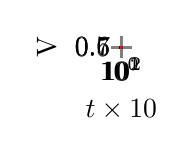
\begin{tikzpicture}

\begin{axis}[%
width=0.951\fwidth,
height=0.75\fwidth,
at={(0\fwidth,0\fwidth)},
scale only axis,
xmode=log,
xmin=1,
xmax=100,
xminorticks=true,
xlabel={$t \times 10$},
ymin=0.45,
ymax=0.7,
ylabel={V},
axis background/.style={fill=white}
]
\addplot [color=blue, line width=2.0pt, forget plot]
  table[row sep=crcr]{%
1	0.457219642968273\\
2	0.592769351348169\\
3	0.628816705720447\\
4	0.62505185351612\\
5	0.628217785699876\\
6	0.639218851111152\\
7	0.630873927371614\\
8	0.636227797683053\\
9	0.638026015044111\\
10	0.636823616047142\\
11	0.632410660316369\\
12	0.633597617267562\\
13	0.636527784056834\\
14	0.637892469025015\\
15	0.633703787028147\\
16	0.636328078671473\\
17	0.637880712599377\\
18	0.634684165215899\\
19	0.629978414138595\\
20	0.628159353629191\\
21	0.637486382196772\\
22	0.630647724209231\\
23	0.636203699395604\\
24	0.632324272807024\\
25	0.643830720098772\\
26	0.633034238724461\\
27	0.635123838924277\\
28	0.636057361395139\\
29	0.642104432395723\\
30	0.63957063775151\\
31	0.636676944667785\\
32	0.638328034343207\\
33	0.642713754763223\\
34	0.638813995795796\\
35	0.637222326954388\\
36	0.641876694490855\\
37	0.637397077631842\\
38	0.641452323880008\\
39	0.639449683802413\\
40	0.63998585281562\\
41	0.645562739043969\\
42	0.638373912813148\\
43	0.63869610092111\\
44	0.639248573866283\\
45	0.64553183974159\\
46	0.64574217834242\\
47	0.647159828876256\\
48	0.642734787921472\\
49	0.645351749272455\\
50	0.647986777824105\\
51	0.648498084835137\\
52	0.641666027891812\\
53	0.649788940171897\\
54	0.644719769480268\\
55	0.642816500136809\\
56	0.648563504192992\\
57	0.647484270514486\\
58	0.646522917641747\\
59	0.646362741362458\\
60	0.64943324763383\\
61	0.650725119238089\\
};
\addplot [color=red, dashed, line width=3.0pt, forget plot]
  table[row sep=crcr]{%
1	0.50533782292246\\
2	0.59699112902373\\
3	0.625888847773672\\
4	0.624084738953654\\
5	0.630607004491168\\
6	0.632831760088705\\
7	0.636757087308418\\
8	0.643065048813731\\
9	0.635831074924727\\
10	0.640172268918583\\
11	0.637618500393285\\
12	0.637063543459606\\
13	0.637801195651245\\
14	0.639132776275881\\
15	0.635237491522697\\
16	0.63711453971561\\
17	0.635829219303754\\
18	0.631722475647075\\
19	0.634325927457996\\
20	0.631533283036592\\
21	0.634408642218423\\
22	0.633190718318277\\
23	0.634003706915972\\
24	0.637844298466811\\
25	0.632637216101121\\
26	0.630133780104625\\
27	0.629845209068525\\
28	0.633468263655565\\
29	0.636356158428604\\
30	0.641203029255701\\
31	0.638991861329888\\
32	0.640709523818283\\
33	0.638816379513034\\
34	0.63827201778754\\
35	0.639309083888535\\
36	0.640322622034011\\
37	0.636038032575251\\
38	0.641624574388145\\
39	0.640674600649206\\
40	0.636610965813643\\
41	0.637518273518509\\
42	0.637490556877938\\
43	0.642085811731694\\
44	0.642900366689167\\
45	0.64514581492819\\
46	0.644982417065964\\
47	0.645169810588366\\
48	0.646840576097694\\
49	0.649222992097267\\
50	0.645768342344984\\
51	0.646975527164982\\
52	0.648342200211879\\
53	0.646810289670806\\
54	0.648718371906363\\
55	0.649127848411779\\
56	0.650500132527732\\
57	0.650312507421561\\
58	0.650414667141449\\
59	0.648262622639421\\
60	0.646204756681934\\
61	0.64655970208432\\
};
\end{axis}
\end{tikzpicture}%
    % This file was created by matlab2tikz.
%
%The latest updates can be retrieved from
%  http://www.mathworks.com/matlabcentral/fileexchange/22022-matlab2tikz-matlab2tikz
%where you can also make suggestions and rate matlab2tikz.
%
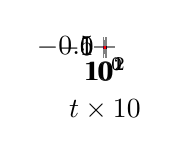
\begin{tikzpicture}

\begin{axis}[%
width=0.951\fwidth,
height=0.75\fwidth,
at={(0\fwidth,0\fwidth)},
scale only axis,
xmode=log,
xmin=1,
xmax=100,
xminorticks=true,
xlabel={$t \times 10$},
ymin=-1.4,
ymax=0,
axis background/.style={fill=white}
]
\addplot [color=blue, line width=2.0pt, forget plot]
  table[row sep=crcr]{%
1	-1.09622117340752\\
2	-0.439738831631238\\
3	-0.477010262732245\\
4	-0.459566994825697\\
5	-0.267438768251134\\
6	-0.261884198822098\\
7	-0.314800806678737\\
8	-0.323934739140698\\
9	-0.204202454295437\\
10	-0.220866546747302\\
11	-0.224784320984486\\
12	-0.174850401323677\\
13	-0.204336810453115\\
14	-0.279220020694667\\
15	-0.304215110722433\\
16	-0.111899168962922\\
17	-0.196698433914746\\
18	-0.212212607848973\\
19	-0.234718297036081\\
20	-0.322668180703975\\
21	-0.286071421580403\\
22	-0.259499649273306\\
23	-0.316375891732036\\
24	-0.273840483206877\\
25	-0.355624719979204\\
26	-0.379757992540423\\
27	-0.288379194513057\\
28	-0.259927407512447\\
29	-0.331340818267421\\
30	-0.342494252379114\\
31	-0.343352143939611\\
32	-0.415313928296665\\
33	-0.422017029459941\\
34	-0.335179784452087\\
35	-0.440060447624601\\
36	-0.514029990888593\\
37	-0.43325890065029\\
38	-0.381527909556519\\
39	-0.357585870240933\\
40	-0.342513238337931\\
41	-0.351232807159593\\
42	-0.491960446194131\\
43	-0.414521352705201\\
44	-0.426725954088604\\
45	-0.442441956965056\\
46	-0.48463572780352\\
47	-0.539087119210198\\
48	-0.444488011314339\\
49	-0.50689510900555\\
50	-0.577616030570053\\
51	-0.438450894005509\\
52	-0.538629948619004\\
53	-0.427097161747581\\
54	-0.449574311025686\\
55	-0.549606168957645\\
56	-0.592101430233288\\
57	-0.633608692550753\\
58	-0.517199531938076\\
59	-0.606102743738442\\
60	-0.513954328614164\\
61	-0.657646711598371\\
};
\addplot [color=red, dashed, line width=3.0pt, forget plot]
  table[row sep=crcr]{%
1	-0.138097439995355\\
2	-0.748893406957869\\
3	-0.82460686564522\\
4	-0.686300787106743\\
5	-0.590927424830682\\
6	-0.644914108373764\\
7	-0.621536393076511\\
8	-0.732227183784745\\
9	-0.678985832465308\\
10	-0.677538882070215\\
11	-0.649492934072179\\
12	-0.626953188541119\\
13	-0.514430272564223\\
14	-0.552610078526062\\
15	-0.651427496731807\\
16	-0.610373827755142\\
17	-0.618730957216695\\
18	-0.62662953336171\\
19	-0.647029602765731\\
20	-0.771071949704786\\
21	-0.881634832338758\\
22	-0.787624432290519\\
23	-0.749027999750425\\
24	-0.768887901516103\\
25	-0.766265274524894\\
26	-0.754819034015115\\
27	-0.682709696959525\\
28	-0.755854713298122\\
29	-0.795893759226808\\
30	-0.87634212964454\\
31	-0.837761717305747\\
32	-0.800158278551069\\
33	-0.788079320268578\\
34	-0.757587585669062\\
35	-0.735977528675732\\
36	-0.792743783163313\\
37	-0.826465829671237\\
38	-0.79949075466688\\
39	-0.763326650871933\\
40	-0.812995026125147\\
41	-0.841258496638301\\
42	-0.811392209795322\\
43	-0.925172456274953\\
44	-0.981952927632142\\
45	-0.903004676499468\\
46	-0.985923064692685\\
47	-1.00004897431729\\
48	-0.981936952406439\\
49	-0.955363797496084\\
50	-0.95804465183494\\
51	-1.02561492499815\\
52	-1.00549051871228\\
53	-0.993986917287425\\
54	-1.03469402307911\\
55	-1.0713271054811\\
56	-1.11079025820582\\
57	-1.12157352569169\\
58	-1.13388551393297\\
59	-1.10161020503734\\
60	-1.10864470943151\\
61	-1.03972034327087\\
};
\end{axis}
\end{tikzpicture}%
    % This file was created by matlab2tikz.
%
%The latest updates can be retrieved from
%  http://www.mathworks.com/matlabcentral/fileexchange/22022-matlab2tikz-matlab2tikz
%where you can also make suggestions and rate matlab2tikz.
%
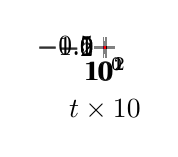
\begin{tikzpicture}

\begin{axis}[%
width=0.951\fwidth,
height=0.75\fwidth,
at={(0\fwidth,0\fwidth)},
scale only axis,
xmode=log,
xmin=1,
xmax=100,
xminorticks=true,
xlabel={$t \times 10$},
ymin=-2,
ymax=-0,
axis background/.style={fill=white}
]
\addplot [color=blue, line width=2.0pt, forget plot]
  table[row sep=crcr]{%
1	-0.00232770753700901\\
2	-1.97313695873102e-05\\
3	-2.37767934892516e-06\\
4	-5.41730805759902e-07\\
5	-7.32149168349694e-08\\
6	-2.39811834130854e-08\\
7	-5.18082968701592e-09\\
8	-5.80788316935145e-09\\
9	-1.76256829256548e-09\\
10	-1.38567073595432e-09\\
11	-2.7766696901406e-10\\
12	-2.3480673996106e-10\\
13	-8.92285754128819e-11\\
14	-1.19961233710043e-10\\
15	-2.67771625177127e-11\\
16	-2.1807283694217e-11\\
17	-9.888893758119e-12\\
18	-2.04587275550225e-11\\
19	-1.00294880288958e-11\\
20	-7.27273007814714e-12\\
21	-2.18409079376077e-12\\
22	-1.90552725474449e-12\\
23	-3.08552681136802e-12\\
24	-1.04407443807789e-12\\
25	-6.89534351010657e-13\\
26	-7.04452116553748e-13\\
27	-5.33265371320719e-13\\
28	-2.21733300835158e-13\\
29	-1.09917521624577e-13\\
30	-1.97092353458009e-13\\
31	-1.06901072975012e-13\\
32	-1.02563119096526e-13\\
33	-8.84436177317179e-14\\
34	-3.79100124163196e-14\\
35	-4.2067887937253e-14\\
36	-2.70027547549659e-14\\
37	-2.66635307650848e-14\\
38	-2.67287785600447e-14\\
39	-2.64342999326352e-14\\
40	-2.65179986462852e-14\\
41	-2.68229872585042e-14\\
42	-2.66997278710527e-14\\
43	-2.69707767201082e-14\\
44	-2.67044068810534e-14\\
45	-2.67210612428623e-14\\
46	-2.65715988911875e-14\\
47	-2.65002787170287e-14\\
48	-2.64873004782108e-14\\
49	-2.61218989350948e-14\\
50	-2.64084264642284e-14\\
51	-2.65721748735916e-14\\
52	-2.66424481150276e-14\\
53	-2.65125945760817e-14\\
54	-2.61390327175519e-14\\
55	-2.63298827930954e-14\\
56	-2.66575354658841e-14\\
57	-2.65806977191069e-14\\
58	-2.63970270948243e-14\\
59	-2.63521868646625e-14\\
60	-2.62708242678811e-14\\
61	-2.67337836777301e-14\\
};
\addplot [color=red, dashed, line width=3.0pt, forget plot]
  table[row sep=crcr]{%
1	-1.61749222996759\\
2	-0.501016985730073\\
3	-0.230141055920469\\
4	-0.211363679210412\\
5	-0.180351722603156\\
6	-0.199490315348852\\
7	-0.167503225130075\\
8	-0.197680427138255\\
9	-0.168326964955281\\
10	-0.108154945624742\\
11	-0.121796007045675\\
12	-0.123244092080481\\
13	-0.120059074298961\\
14	-0.12768082663036\\
15	-0.118695747205944\\
16	-0.14620525838291\\
17	-0.156154755993665\\
18	-0.15210970699618\\
19	-0.171018095781681\\
20	-0.159637204861449\\
21	-0.147168529193469\\
22	-0.282154360398568\\
23	-0.245469097598784\\
24	-0.252947839856794\\
25	-0.242482705863201\\
26	-0.244915288625687\\
27	-0.224359689620484\\
28	-0.214533978554422\\
29	-0.216114585568234\\
30	-0.208860180236654\\
31	-0.221529291908727\\
32	-0.205563531932023\\
33	-0.233055721377914\\
34	-0.23298981535382\\
35	-0.215062245554676\\
36	-0.226954153936872\\
37	-0.222039885512241\\
38	-0.198543948266946\\
39	-0.191065849011378\\
40	-0.189777971418282\\
41	-0.188793398961995\\
42	-0.190732460573578\\
43	-0.185246409681183\\
44	-0.184603807555449\\
45	-0.188647955865062\\
46	-0.191033781025243\\
47	-0.179745728112148\\
48	-0.178803266307534\\
49	-0.163926246089407\\
50	-0.173423292392264\\
51	-0.179302094659936\\
52	-0.181333239906458\\
53	-0.177046092214897\\
54	-0.184951112414626\\
55	-0.181338109208384\\
56	-0.147815635344293\\
57	-0.149881515239679\\
58	-0.14463523042435\\
59	-0.144488753661275\\
60	-0.150296785419916\\
61	-0.157708726945062\\
};
\end{axis}
\end{tikzpicture}%
  }
  \textbf{\alert<2>{Online setting: data seen depends on decisions}}
  \scalebox{0.35}{
    % This file was created by matlab2tikz.
%
%The latest updates can be retrieved from
%  http://www.mathworks.com/matlabcentral/fileexchange/22022-matlab2tikz-matlab2tikz
%where you can also make suggestions and rate matlab2tikz.
%
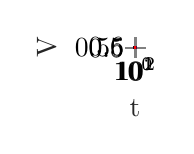
\begin{tikzpicture}

\begin{axis}[%
width=0.951\fwidth,
height=0.75\fwidth,
at={(0\fwidth,0\fwidth)},
scale only axis,
xmode=log,
xmin=1,
xmax=100,
xminorticks=true,
xlabel style={font=\color{white!15!black}},
xlabel={t},
ymin=0.5,
ymax=0.64,
ylabel style={font=\color{white!15!black}},
ylabel={V},
axis background/.style={fill=white}
]
\addplot [color=blue, line width=2.0pt, forget plot]
  table[row sep=crcr]{%
1	0.533404412801252\\
2	0.567059367237681\\
3	0.574983684728794\\
4	0.595440941591605\\
5	0.597329784902714\\
6	0.598376899476387\\
7	0.608381899604062\\
8	0.614299903055019\\
9	0.614682328515722\\
10	0.622047920597586\\
11	0.624110283420211\\
12	0.623040076545587\\
13	0.622922815525939\\
14	0.622693703044924\\
15	0.624972493335543\\
16	0.623768267741923\\
17	0.625076223581217\\
18	0.624417108492841\\
19	0.624469368091222\\
20	0.626122024040929\\
21	0.627990230164747\\
22	0.627328710101433\\
23	0.627229984116765\\
24	0.627284500665436\\
25	0.628167660760683\\
26	0.62745907557843\\
27	0.627233400174376\\
28	0.626561170176999\\
29	0.626140421275828\\
30	0.627206627096838\\
31	0.626985313402765\\
32	0.627098543124935\\
33	0.626653517790801\\
34	0.62669323165553\\
35	0.626164136918594\\
36	0.625226096500675\\
37	0.624375614738648\\
38	0.626043052672986\\
39	0.625037401619658\\
40	0.624754173295781\\
41	0.625734326489491\\
42	0.624858959455676\\
43	0.624748862220927\\
44	0.625474170196668\\
45	0.624772055502031\\
46	0.624434789925371\\
47	0.624134265867323\\
48	0.624465786011358\\
49	0.62488377850369\\
50	0.624799243863898\\
51	0.623188769161788\\
52	0.622787015457619\\
53	0.625093107691527\\
54	0.62416250160529\\
55	0.624845855606283\\
56	0.625039701294087\\
57	0.625218860435963\\
58	0.626623043783051\\
59	0.626765171689463\\
60	0.626873002508487\\
};
\addplot [color=red, dashed, line width=3.0pt, forget plot]
  table[row sep=crcr]{%
1	0.537691550449067\\
2	0.52692425944197\\
3	0.51952806147473\\
4	0.516060917995437\\
5	0.525734464151558\\
6	0.526857982759685\\
7	0.527688486772251\\
8	0.553006242367054\\
9	0.580639537966924\\
10	0.583055435798432\\
11	0.583845485337254\\
12	0.585535021854244\\
13	0.589716220033718\\
14	0.591727972382982\\
15	0.592321109916687\\
16	0.593212336283605\\
17	0.59331788850473\\
18	0.592639117087132\\
19	0.594276492899578\\
20	0.593631864589812\\
21	0.593134373439542\\
22	0.592526975573227\\
23	0.59343823978082\\
24	0.59471503376963\\
25	0.594382031634667\\
26	0.59347186036185\\
27	0.594295880998185\\
28	0.592974355499971\\
29	0.594610054709994\\
30	0.594316274450942\\
31	0.59587687254927\\
32	0.594384171167264\\
33	0.59368169358206\\
34	0.593672061191477\\
35	0.59309575835021\\
36	0.591830149985295\\
37	0.592248365155305\\
38	0.592785655298101\\
39	0.592284775003569\\
40	0.591763395381349\\
41	0.591416781456517\\
42	0.593000957180953\\
43	0.591369641506618\\
44	0.592580298295271\\
45	0.592677941655292\\
46	0.591707641469623\\
47	0.592929785718232\\
48	0.591688464121018\\
49	0.591343754331541\\
50	0.589724575501398\\
51	0.590358577218326\\
52	0.590327436945083\\
53	0.590665615799822\\
54	0.595774337247164\\
55	0.595592315397091\\
56	0.595804057900644\\
57	0.59578874458756\\
58	0.596457066440588\\
59	0.597530717491227\\
60	0.597648444447298\\
};
\end{axis}
\end{tikzpicture}%
    % This file was created by matlab2tikz.
%
%The latest updates can be retrieved from
%  http://www.mathworks.com/matlabcentral/fileexchange/22022-matlab2tikz-matlab2tikz
%where you can also make suggestions and rate matlab2tikz.
%
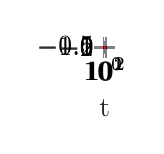
\begin{tikzpicture}

\begin{axis}[%
width=0.951\fwidth,
height=0.75\fwidth,
at={(0\fwidth,0\fwidth)},
scale only axis,
xmode=log,
xmin=1,
xmax=100,
xminorticks=true,
xlabel style={font=\color{white!15!black}},
xlabel={t},
ymin=-2,
ymax=-0,
axis background/.style={fill=white}
]
\addplot [color=blue, line width=2.0pt, forget plot]
  table[row sep=crcr]{%
1	-0.139557730363354\\
2	-0.238920667169255\\
3	-0.0997916326764938\\
4	-0.182229548458017\\
5	-0.205267446075831\\
6	-0.279826712648142\\
7	-0.332249305176689\\
8	-0.323237535828966\\
9	-0.334848601807552\\
10	-0.312990041492882\\
11	-0.324619975130561\\
12	-0.328870423071226\\
13	-0.313326571427902\\
14	-0.319808076558834\\
15	-0.30709006893331\\
16	-0.317914410723469\\
17	-0.331045983578041\\
18	-0.342385254226511\\
19	-0.358246869022327\\
20	-0.369248314322897\\
21	-0.377973473224499\\
22	-0.415440383538921\\
23	-0.38990705668132\\
24	-0.36686729244785\\
25	-0.375042658748737\\
26	-0.366006828119552\\
27	-0.383213880975782\\
28	-0.386114407046102\\
29	-0.380250046047834\\
30	-0.399759884881641\\
31	-0.437509783568944\\
32	-0.439357807489347\\
33	-0.443493819937183\\
34	-0.43823346019647\\
35	-0.448743781654721\\
36	-0.46057428729186\\
37	-0.465056676021326\\
38	-0.455095054216753\\
39	-0.463602980734887\\
40	-0.497134299702848\\
41	-0.456405475996486\\
42	-0.461607953659762\\
43	-0.467431543238734\\
44	-0.481699178907957\\
45	-0.497488409531242\\
46	-0.491566651303831\\
47	-0.489462737779279\\
48	-0.508962806633321\\
49	-0.497498682067592\\
50	-0.49354033957002\\
51	-0.497912056057912\\
52	-0.496093017678467\\
53	-0.505412512936155\\
54	-0.503382028933859\\
55	-0.52416214442533\\
56	-0.522603926762207\\
57	-0.544550008258789\\
58	-0.532153628446791\\
59	-0.520440892587704\\
60	-0.532834541878595\\
};
\addplot [color=red, dashed, line width=3.0pt, forget plot]
  table[row sep=crcr]{%
1	-0.759593109224573\\
2	-0.851910476827388\\
3	-0.931248398068395\\
4	-0.899099878562075\\
5	-0.7313280766324\\
6	-0.866207448068707\\
7	-0.990998285997023\\
8	-1.0272085536674\\
9	-1.04372995832914\\
10	-1.07714261034557\\
11	-1.07998626920429\\
12	-1.1166916978057\\
13	-1.09921640121892\\
14	-1.11870116207787\\
15	-1.14149626270435\\
16	-1.13602637450519\\
17	-1.19256259507435\\
18	-1.18855636890274\\
19	-1.16210813506113\\
20	-1.19312997954371\\
21	-1.16517236023971\\
22	-1.09072259193678\\
23	-1.07693553149219\\
24	-1.09320599058905\\
25	-1.12532578022789\\
26	-1.14329006175479\\
27	-1.17276265772882\\
28	-1.15208234230952\\
29	-1.18083392582687\\
30	-1.20703772222562\\
31	-1.22005481633382\\
32	-1.21874241865254\\
33	-1.26208489068812\\
34	-1.22937949908594\\
35	-1.26117480001724\\
36	-1.2690068818918\\
37	-1.26700389402755\\
38	-1.27433797411748\\
39	-1.28632957244659\\
40	-1.31543453440127\\
41	-1.32705144995612\\
42	-1.33602820271486\\
43	-1.3294527996667\\
44	-1.31996093710498\\
45	-1.32018176557428\\
46	-1.32494053379554\\
47	-1.33735592039034\\
48	-1.34339401770564\\
49	-1.33957969692087\\
50	-1.35053901850318\\
51	-1.34476886404259\\
52	-1.37641480485034\\
53	-1.35196334938376\\
54	-1.38384298807204\\
55	-1.40343614175046\\
56	-1.38977437984097\\
57	-1.37450630646827\\
58	-1.39440827751891\\
59	-1.41230095819747\\
60	-1.42020708154538\\
};
\end{axis}
\end{tikzpicture}%
    % This file was created by matlab2tikz.
%
%The latest updates can be retrieved from
%  http://www.mathworks.com/matlabcentral/fileexchange/22022-matlab2tikz-matlab2tikz
%where you can also make suggestions and rate matlab2tikz.
%
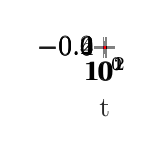
\begin{tikzpicture}

\begin{axis}[%
width=0.951\fwidth,
height=0.75\fwidth,
at={(0\fwidth,0\fwidth)},
scale only axis,
xmode=log,
xmin=1,
xmax=100,
xminorticks=true,
xlabel style={font=\color{white!15!black}},
xlabel={t},
ymin=-0.7,
ymax=-0,
axis background/.style={fill=white}
]
\addplot [color=blue, line width=2.0pt, forget plot]
  table[row sep=crcr]{%
1	-0.015991389253571\\
2	-8.07710251594484e-14\\
3	-2.59936539286564e-14\\
4	-2.60348785986828e-14\\
5	-2.60224200315188e-14\\
6	-2.59820525418944e-14\\
7	-2.59965938614317e-14\\
8	-2.60060611148019e-14\\
9	-2.59506757310226e-14\\
10	-2.58498969706858e-14\\
11	-2.58919987094477e-14\\
12	-2.59483989064604e-14\\
13	-2.595303495495e-14\\
14	-2.59150661948695e-14\\
15	-2.59299891535716e-14\\
16	-2.59070821300713e-14\\
17	-2.58991891382556e-14\\
18	-2.59151399206172e-14\\
19	-2.59036430407802e-14\\
20	-2.59284539232954e-14\\
21	-2.58943058916708e-14\\
22	-2.58760956319817e-14\\
23	-2.59459746304027e-14\\
24	-2.59175295022054e-14\\
25	-2.59825035699981e-14\\
26	-2.58938635371844e-14\\
27	-2.58310058320324e-14\\
28	-2.58420733678091e-14\\
29	-2.58783117412223e-14\\
30	-2.58440162581022e-14\\
31	-2.58429971080601e-14\\
32	-2.58351474843313e-14\\
33	-2.5869000612965e-14\\
34	-2.59091421141991e-14\\
35	-2.58739836061497e-14\\
36	-2.59131536622373e-14\\
37	-2.5829626726869e-14\\
38	-2.58271634195331e-14\\
39	-2.59047142325266e-14\\
40	-2.58443241715192e-14\\
41	-2.58396707757949e-14\\
42	-2.58215472522796e-14\\
43	-2.57845499373457e-14\\
44	-2.57547777456893e-14\\
45	-2.58627556084514e-14\\
46	-2.58798513083072e-14\\
47	-2.58572825558847e-14\\
48	-2.58443111610931e-14\\
49	-2.58880695607746e-14\\
50	-2.60105757326481e-14\\
51	-2.59875602889306e-14\\
52	-2.60626044265013e-14\\
53	-2.58993130083538e-14\\
54	-2.5891459860968e-14\\
55	-2.58690168759975e-14\\
56	-2.59416063798498e-14\\
57	-2.59585459545927e-14\\
58	-2.5878549181498e-14\\
59	-2.57975375951699e-14\\
60	-2.59211019483637e-14\\
};
\addplot [color=red, dashed, line width=3.0pt, forget plot]
  table[row sep=crcr]{%
1	-0.677360003940489\\
2	-0.319188261527385\\
3	-0.238573589451842\\
4	-0.200742996733391\\
5	-0.188801791973792\\
6	-0.157848169305053\\
7	-0.147363581418297\\
8	-0.151590768638053\\
9	-0.164301512639608\\
10	-0.198659955535581\\
11	-0.185472157543024\\
12	-0.189488927671266\\
13	-0.156665545344133\\
14	-0.141346012616817\\
15	-0.142828076379696\\
16	-0.143980205895357\\
17	-0.14494774267628\\
18	-0.145557100703442\\
19	-0.14609092309342\\
20	-0.137324402147981\\
21	-0.134764797162596\\
22	-0.140554448009126\\
23	-0.142899121135694\\
24	-0.143712900049346\\
25	-0.138774590312461\\
26	-0.13836037206626\\
27	-0.135282806601259\\
28	-0.149453779259262\\
29	-0.147470735870606\\
30	-0.154207490480793\\
31	-0.155796490189568\\
32	-0.158732344859596\\
33	-0.163488711963298\\
34	-0.166258826196893\\
35	-0.172242532053593\\
36	-0.168635982124319\\
37	-0.170553091320478\\
38	-0.171303646165357\\
39	-0.185837521836149\\
40	-0.180259389616782\\
41	-0.174263442475532\\
42	-0.162013378918257\\
43	-0.167114368469105\\
44	-0.169568455307836\\
45	-0.173271142995335\\
46	-0.191054413001525\\
47	-0.202850261177353\\
48	-0.209494088522992\\
49	-0.213131370871494\\
50	-0.211058535404276\\
51	-0.207988868337055\\
52	-0.20444195101075\\
53	-0.209951638264728\\
54	-0.218554354326512\\
55	-0.227181804255464\\
56	-0.233332843632866\\
57	-0.240435706083566\\
58	-0.246103352664639\\
59	-0.243526218854078\\
60	-0.236038905669898\\
};
\end{axis}
\end{tikzpicture}%
  }
  \fbox{\parbox{16em}{
    \begin{itemize}
    \item Observe $x_t$.
    \item Take action $a_t$.
    \item Observe $y_t$\only<2>{ if $a_t = 1$}.
    \end{itemize}
  }}
  \begin{tikzpicture}

  \begin{axis}[%
    hide axis,
    xmin=10,
    xmax=50,
    ymin=0,
    ymax=0.4,
    legend style={draw=white!15!black,legend cell align=left}
    ]
    \addlegendimage{color=mycolor1, line width=2.0pt}
    \addlegendentry{Bayes};
    \addlegendimage{color=mycolor2, dashed, line width=3.0pt};
    \addlegendentry{Marginal};
  \end{axis}
\end{tikzpicture}


  \note<1>{We also experimented with the COMPAS data. Here there is no ground truth, so we measure fairness and utility with respect to the empirical distribution on a hold-out set.
    In the top, we see the results for the offline setting, where the data that we see at each time step is the same irrespective of our decisions. We see that the results are similar to those of the synthetic data, withe the difference that we converge to something that is different from the empirical distribution on the hold-out set, so it is harder to measure fairness. Again, the Bayesian approach is better than the marginal, apart from the case when $\lambda=0$, where we do not care about fairness. }
  \note<2>{In the online setting, we observe $x$, then take an action $a$ and only observe the outcome if our action was to release the individual. Thus, just as in the experiment design and bandit setting, our decisions affect the data we see. Here the  difference between the two approaches is more obvious. This is because the Bayesian approach explicitly takes the available model information into account. Hence, there is an advantage even in the case where we do not care about fairness at all. This shows rather clearly that using a certainty equivalence principle is not a very good idea.}

\end{frame}
\begin{frame}
  \frametitle{Summary}
  
  \begin{itemize}
  \item Existing criteria hard to satisfy.
  \item Bayesian framework:
    \begin{itemize}
    \item Incorporates model uncertainty.
    \item Considers informational aspects.
    \item Lower fairness violation.
    \end{itemize}
  \end{itemize}
  
  \begin{block}{Future work}
    \begin{itemize}
    \item<alert@1> Non-myopic sequential decision making.
    \item<alert@2> Approximate Bayesian methods.
    \end{itemize}
  \end{block}
  \includegraphics[height=0.1\textwidth]{../figures/me-recent} \hspace{1em}
  \only<1>{
    \includegraphics[height=0.1\textwidth]{../figures/parkes} \hspace{1em}
    \includegraphics[height=0.1\textwidth]{../figures/magdalena}
    \hspace{1em}
    \includegraphics[height=0.1\textwidth]{../figures/aleksander}
    \hspace{1em}
    \includegraphics[height=0.1\textwidth]{../figures/fabio}
    \hspace{1em}
    \includegraphics[height=0.1\textwidth]{../figures/oslo}
    \hspace{1em}
    \includegraphics[height=0.1\textwidth]{../figures/harvard}
  }
  \only<2>{
    \includegraphics[height=0.1\textwidth]{../figures/amanda-belfrage} \hspace{1em}
    \includegraphics[height=0.1\textwidth]{../figures/david-berg} \hspace{1em}
    \includegraphics[height=0.1\textwidth]{../figures/chalmers_dark}
  }
\end{frame}

%%% Local Variables:
%%% mode: latex
%%% TeX-master: "fairness-presentation-vetenskap"
%%% End:
